\documentclass[tikz,border=10pt]{standalone}
\begin{document}
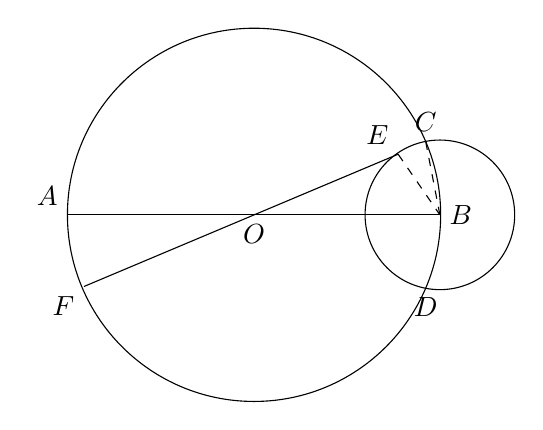
\begin{tikzpicture}
\coordinate (O) at (3.04,0);
\coordinate (A) at (0.67,0);
\coordinate (B) at (5.40,0);
\coordinate (C) at (5.22,0.93);
\coordinate (D) at (5.22,-0.93);
\coordinate (E) at (4.87,0.77);
\coordinate (F) at (0.88,-0.91);

\draw (O) circle (2.37);
\draw (B) circle (0.95);
\draw (A) -- (B);
\draw (F) -- (E);
\draw[dashed] (E) -- (B);
\draw[dashed] (C) -- (B);

\node[above left] at (A) {$A$};
\node[right] at (B) {$B$};
\node[above] at (C) {$C$};
\node[below] at (D) {$D$};
\node[above left] at (E) {$E$};
\node[below left] at (F) {$F$};
\node[below] at (O) {$O$};
\end{tikzpicture}
\end{document}
